\section{Entwurfsphase}


\subsection{Zielplatform}
Wie aus der Sektion Projektziel entnommen werden kann, soll das Projekt als Kommandozeilenprogramm
implementiert werden. Aufgrund der Anforderungen aus dem Lastenheft, welches Speicherperformanz sowie Geschwindigkeit fordert,
fiel die Entscheidung der Programmiersprache recht schnell. C ist eine Hochsprache, welche effizient und extrem schnell
die geforderten Berechnungen ausführen kann, und dem Programmierer eine ideale Schnittstelle bietet, effizient im Speicher zu agieren.
Um jedoch persönliche Erfahrungen und Ansichten zu verifizieren, wurden diverse weitere Sprachen anhand einer
Nutzwertanalyse verglichen. Die wichtigste Rolle spielten hierbei folgende Kriterien:
\begin{itemize}
    \item Performanz - Geschwindigkeit der Sprache in der HPC Domäne
    \item Speichereffizienz - Der Fußabdruck der Sprache, sowie deren Objekte im Speicher soll möglichst gering sein
    \item Dokumentation - Bibliotheken und Module sollten gut und einsehbar dokumentiert sein.
    \item Systemische Vorraussetzungen - Anzahl und Aufwand der Vorraussetzungen um die Sprache zu nutzen
\end{itemize}

Die Ergebnisse dieses Vergleichs wurden in der Nutzwertanalyse \ref{nwa_sprachen} präsentiert.\par
Letztendlich wurde an der initialen Entscheidung, die Sprache C zu nutzen, festgehalten.

\subsection{Algorithmusdesign}
In Zusammenarbeit mit der Abteilung für Datenverarbeitung hat der Autor einen simplen
Pseudocode für die grundlegende Logik des Algorithmus entwickelt, welcher als Ausgangspunkt
für die weitere Entwicklung genutzt wurde. Dieser wurde vom Autor in Form eines
Aktivitätsdiagramm\ref{programmlogik} im Anhang, visualisiert.
Der Pseudo code ist ebenfalls auf Seite X im Anhang einsehbar.
Hierbei wurden sogenannte QGramme verwendet - diese verstehen sich als
Teilstring eines Strings der Länge Q.



\subsection{Architekturdesign}
Das Projekt besteht aus 2 Header-Dateien und einer main.c. Die Header Dateien
beinhalten zum einen die Algorithmus-spezifischen Funktionen zum Vergleich von
Strings, zum anderen eine open-source Hashmap implementation.

\begin{figure}[!htp]
	\label{folderstruct}
	\caption{Übersicht der Ordnerstruktur. Hochauflösung im Anhang.}
	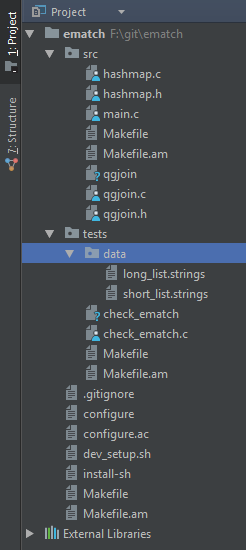
\includegraphics[width=0.5\textwidth]{folder_struct}
\end{figure}

Auf programmatischer Ebene wurde das Programm in zwei Abschnitte unterteilt:
\begin{itemize}
    \item \textbf{Vorbereitung} \\
    Hier werden Daten aus der ersten Datei geladen und benötigte Datenstrukturen im Speicher angefordert.
    Variablen werden initialisiert und der QGram Pool erstellt.
    \item \textbf{Ausführung} \\
    Das zweite Set an Daten wird über einen File Pointer referenziert und die
    Strings werden Zeile für Zeile ausgelesen, ihre QGramme mit denen im Schritt
    Vorbereitung erstellten verglichen und bei einer genügenden Übereinstimmung
    über STDOUT ausgegeben.
\end{itemize}

Hieraus ergaben sich 8 Sub-komponenten, welche einer Implementierung bedurften:


\begin{itemize}
    \item \textbf{Vorbereitung}:
    \begin{itemize}
        \item \textbf{S}: Eine Menge aller Strings aus der ersten Liste bzw Datei
        \item \textbf{Q}: Eine Menge aller QGramme, welche sich aus denjeweils einzelnen Strings in S generieren lassen
    \end{itemize}

    \item Ausführung
    \begin{itemize}
        \item \textbf{I}: Eine Menge, welche die gleiche Größe wie S ist und die
        Anzahl der Qgramme zählt, welche für den jeweiligen Index eines Strings in
        S passen.
        \item \textbf{f}: Eine Referenz zur zweiten Liste, von der wir zur vergleichende
        Strings holen können
        \item \textbf{T}: Eine Menge der Qgramme in der zur Zeit ausgelesenen Zeile
        \item \textbf{M}: Eine Menge der Indizes von Strings, welche auf die QGramme
        T am besten passen
    \end{itemize}
\end{itemize}

Mit Ausname von Q und M können alle Datenstrukturen mit den geläufigen C
Datentypen ausgedrückt werden.

Für die Strukturen Q und M mussten jedoch neue Datenstrukturen
erstellt werden. Für Q bot sich hier eine Hashmap an - prinzipiell besteht
hier zwar ein höherer Speicheraufwand, dieser ist jedoch abschätzbar, da die
maximale Anzahl an möglichen Key-Value Einträgen begrenzt ist. Der darausfolgende
O(1) Suchaufwand zum vergleich von Qgramme ist ein unschätzbarer Vorteil in der
späteren Ausführung. Auch hier wurde wiederum eine Nutzwertanalyse\ref{nwa_datentyp} durchgeführt,
um sicherzustellen dass die persönlichen Annahmen des Autors mit den technischen
Gegebenheiten übereinstimmen.
Hierzu wurden verschiedene Datenstrukturen nach folgenden Kriterien bewertet:

\begin{enumerate}
    \item \textbf{Speicheraufwand} \\
    Da laut Vorgabe maximal 32GB zur Ausführung des Programms zur Verfügung stehen,
    sollte der Speicherverbrauch natürlich so gering wie möglich sein. Da jedoch
    die maximale Datengröße aufgrund der 7-Bit ASCII Kodierung der Strings
    bekannt ist, ist dieses Kriterium am geringsten gewichtet worden.\par
    \item \textbf{Schnelligkeit Einfügen-Befehl} \\
    Das Erstellen der Datenstruktur sollte der größte rechnerische Aufwand im
    ersten Schritt des Programms sein. Deshalb sollte hier möglichst effizient gearbeitet und
    der Aufwand entsprechend optimiert sein.\par
    \item \textbf{Schnelligkeit Such-Befehl} \\
    Einen Wert aus der Datenstruktur abzufragen sollte nach möglichkeit in
    Richtung von Aufwand O(1) gehen, da dies mehrfach während des Stringvergleichs
    gebraucht wird. Deshalb ist dieses Kriterium auch am höchsten Gewichtet worden,
    da hier die größten Engpässe entstehen können.\par

\end{enumerate}

Für M wird eine dynamisch wachsende Array benötigt, da die Anzahl der passenden
QGramme je nach String variiert. Da die Anzahl der möglichen Zeichen pro QGramm von unserem
verwendeten Zeichensatz begrenzt ist (7-Bit ASCII), konnte eine begründete Annahme
über die Verteilung der QGramme in der Menge der Strings gemacht werden. Diese wurde anhand eines
Graphen\ref{qgram_verteilung} dargestellt. Die Verteilung stellt als Quantil die 
Menge an Qgrammen der String Daten dar.
Anhand dieser Analyse konnte eine optimale Startgröße festlegt werden, sodass in etwa der Hälfte der Fälle
erwartet werden kann, dass das Array nicht vergrößert werden muss, und somit die
Speicherzuweisungen minimiert werden.

\begin{figure}[!htp]
	\label{qgram_verteilung_klein}
	\caption{Qgramverteilung der Daten. Hochauflösung im Anhang.}
	\includegraphics[width=.25\textwidth]{multiplicity_of_qgrams}
\end{figure}

In Einklang mit der test-getriebenen Entwicklung wurde von Anfang an ein Hauptaugenmerk
auf die möglichst granulare Entwicklung des Codes gelegt. So wurden die Schritte
des Algorithmus in jweils mindestens einen Test und eine dazugehörige Funktion unterteilt \ref{listing_tests}.
Auch wurden für jeden selbsterstellten Datentypen und dazugehörige Funktionen
ebenfalls zunächst ein Test geschrieben.



\subsection{Entwurf der Benutzeroberfläche}
Der GNU Codingstandard\cite{gnuCodingStandard},
sowie die POSIX Utility Guidelines\cite{posixGuidelines}
spezifizieren standardisierte Parameternamen und Funktionen eines Programms, sowie
deren erwartete Funktion. Da es sich bei der Zielgruppe um erfahrene Linuxnutzer handelt, wurde das
Kommandozeilenprogramm nach diesen Standards auch entwickelt. Ein Auszug dieser
Vorgaben befindet sich im Anhang auf Seite X.\par

Auf eine grafische Nutzeroberfläche wird verzichetet, da die bevorzugte
Oberfläche der Endnutzer die Kommandozeile ist.

\subsection{Datenmodell}
Aufgrund der Natur der Daten ist das Datenmodell für das Projekt trivial. Es besteht aus einer
einspaltigen Tabelle, welche in Relation zu sich selbst steht. Aus diesen Gründen wird auf eine weitere Ausführung des 
Modells verzichtet - die UML Grafik des Modells kann jedoch im Anhang\ref{fig:datenmodell} eingesehen werden.

Es ist zu klärifizieren, dass die GA Financial Solution kaum bis gar nicht Datenbanksysteme wie
MySQL, MongoDB u.Ä. nutzt. Stattdessen werden komprimmierte csv Dateien verwendet, welche
meist nur aus 3 Zeilen (Zeitstempel, Typ und Wert) bestehen. Dies ergibt sich aus
der negativen Erfahrung mit Datenbankmanagementsystemen und der Vereinfachung des Workflows durch
die Nutzung von CSV Daten in Kombination mit der hauseigenen CLI Toolchain.


\subsection{Geschäftslogik}
Zur Veranschaulichung der beisherigen Geschäftslogik, wurde eine Aktivitätendiagramm\ref{fig:geschäftslogikAlt} 
erstellt.Wie dort zu erkennen ist,
ist die Abholung der Daten von Anbietern automatisiert, die Verarbeitung jedoch nicht.
Diese geschieht bei Bedarf und erfordert u.A. die Vorsortierung der Daten in handhabbare
Datensätze, welche einfacher und in angemessener Zeit von unseren 4 Kern Maschinen
berechnet werden können. Zudem kommt noch eine erforderliche manuelle Überprüfung
der Ergebnisse. Die Darausentstehenden Daten werden schließlich für das derzeitig entwickelte Projekt
genutzt und schlussendlich wieder verworfen, da die Datensätze hoch parametrisiert sind,
und nicht zur generellen Nutzung innerhalb der Firma eignen.\par



\subsection{Pflichtenheft / Datenverarbeitungskonzept}
Abschließend zur Entwurfsphase wurde ein Pflichtenheft erstellt und dieses als
Roter Faden für das Projekt der Abteilung für Datenverarbeitung vorgelegt. Wie im
Projektmanagement üblich, baut dieses auf dem Lastenheft auf.
Ein Auszug des Pflichtenhefts\ref{anhang:pflichtenheft} befindet sich im Anhang.
